% ============================================================
% Support de soutenance — Projet numérique de physique moderne
% Effet tunnel et temps de traversée d'une barrière de potentiel
% Compilation : pdflatex presentation.tex (deux passes)
% ============================================================
\documentclass[10pt,aspectratio=169]{beamer}

\usepackage[utf8]{inputenc}
\usepackage[T1]{fontenc}
\usepackage[french]{babel}
\usepackage{amsmath,amssymb}
\usepackage{graphicx}
\usepackage{booktabs}
\usepackage[sfdefault,light]{FiraSans}
\usepackage{newtxsf}

\graphicspath{{figures/}}

% ----- Style fait main : sobre, papier ivoire, accent bordeaux -----
\definecolor{encre}{HTML}{2B2B2B}      % texte principal
\definecolor{bordeaux}{HTML}{7D1D21}   % accent
\definecolor{papier}{HTML}{FBFAF7}     % fond
\definecolor{grisdoux}{HTML}{8A8680}   % éléments secondaires
\definecolor{filet}{HTML}{D8D3CA}      % règles fines, fonds de bloc

\setbeamercolor{background canvas}{bg=papier}
\setbeamercolor{normal text}{fg=encre}
\setbeamercolor{structure}{fg=bordeaux}
\setbeamercolor{alerted text}{fg=bordeaux}

\setbeamertemplate{navigation symbols}{}
\setbeamerfont{frametitle}{size=\Large,series=\bfseries}
\setbeamercolor{frametitle}{fg=encre}

% Titre de diapo : texte sombre + filet bordeaux court
\setbeamertemplate{frametitle}{%
  \vspace{0.9em}%
  {\usebeamerfont{frametitle}\insertframetitle\par}%
  \vspace{0.25em}%
  {\color{bordeaux}\rule{2.2em}{1.6pt}}\par
  \vspace{0.2em}%
}

% Pied de page : discret, en bas à droite
\setbeamertemplate{footline}{%
  \hfill{\color{grisdoux}\scriptsize\insertshorttitle\ \textperiodcentered\
  \insertframenumber/\inserttotalframenumber}\hspace{1.2em}\vspace{0.6em}%
}

% Puces : tirets, sous-puces : petits traits
\setbeamertemplate{itemize item}{\color{bordeaux}\textbf{--}}
\setbeamertemplate{itemize subitem}{\color{grisdoux}\textbf{--}}
\setbeamertemplate{enumerate item}{\color{bordeaux}\insertenumlabel.}
\setbeamercolor{itemize item}{fg=bordeaux}

% Blocs : plats, fond discret, titre bordeaux sans barre colorée
\setbeamertemplate{blocks}[default]
\setbeamercolor{block title}{fg=bordeaux,bg=filet!35}
\setbeamercolor{block body}{fg=encre,bg=filet!35}
\setbeamerfont{block title}{series=\bfseries,size=\normalsize}

% Page de titre minimaliste
\setbeamertemplate{title page}{%
  \vfill
  {\color{grisdoux}\small\insertinstitute\par}
  \vspace{0.4em}
  {\color{bordeaux}\rule{3em}{1.6pt}}\par
  \vspace{0.9em}
  {\LARGE\bfseries\inserttitle\par}
  \vspace{0.5em}
  {\large\color{encre}\insertsubtitle\par}
  \vspace{2.2em}
  {\normalsize\insertauthor\par}
  \vspace{0.3em}
  {\small\color{grisdoux}\insertdate\par}
  \vfill
}

% Raccourcis
\newcommand{\hb}{\hbar}
\newcommand{\eg}{\,\mathrm{e}}

\title[Effet tunnel et temps de traversée]
      {Effet tunnel et temps de traversée\\d'une barrière de potentiel}
\subtitle{Dynamique d'un paquet d'ondes gaussien à une dimension}
\author{Myriam Bensaid, Sheryne Ouarghi, Mattéo Knopes}
\institute{Projet numérique — Physique moderne 2025--2026}
\date{Soutenance — juin 2026}

\begin{document}

% ------------------------------------------------------------
\begin{frame}
  \titlepage
\end{frame}

% ------------------------------------------------------------
\begin{frame}{Problématique}
  \begin{block}{Question centrale}
    Combien de temps met une particule quantique pour traverser une
    barrière de potentiel qu'elle n'a \emph{classiquement} pas le droit de franchir ?
  \end{block}
  \vspace{0.5em}
  \textbf{Démarche du projet :}
  \begin{enumerate}
    \item Construire un paquet d'ondes gaussien et comprendre sa dynamique libre ;
    \item Déterminer les états stationnaires de la barrière rectangulaire
          (transmission $|T|^2$, phase $\varphi_T$) ;
    \item Résoudre numériquement l'équation de Schrödinger dépendante du temps
          (schéma de Crank--Nicolson) ;
    \item Mesurer le temps de traversée et le comparer à la prédiction
          théorique (temps de groupe de Hartman) ;
    \item Étudier l'influence de la barrière ($a$, $V_0$) \emph{et} du paquet
          ($k_0$, $a_{\rm wp}$) sur ce temps.
  \end{enumerate}
  \vspace{0.5em}
  Unités adimensionnées : $\hb = m = 1$.
\end{frame}

% ------------------------------------------------------------
\begin{frame}{Le paquet d'ondes gaussien}
  Une particule localisée = superposition d'ondes planes :
  \[
    \psi(x,t) = \frac{1}{\sqrt{2\pi}} \int g(k)\,\eg^{i(kx - \omega(k)t)}\,dk,
    \qquad \omega(k) = \frac{\hb k^2}{2m}
  \]
  avec un poids gaussien $g(k) \propto \eg^{-a_{\rm wp}(k-k_0)^2}$ centré en $k_0$.

  \begin{columns}[T]
    \begin{column}{0.48\textwidth}
      \textbf{Propriétés clés :}
      \begin{itemize}
        \item vitesse de groupe $v_g = \hb k_0/m$ \\
              (vitesse du centre du paquet) ;
        \item vitesse de phase $v_\varphi = v_g/2$ ;
        \item largeur spectrale $\Delta k = \dfrac{1}{2\sqrt{a_{\rm wp}}}$ \\
              $\Rightarrow$ étroit en $x$ $\Leftrightarrow$ large en $k$ ;
        \item étalement (dispersion) au cours du temps.
      \end{itemize}
    \end{column}
    \begin{column}{0.48\textwidth}
      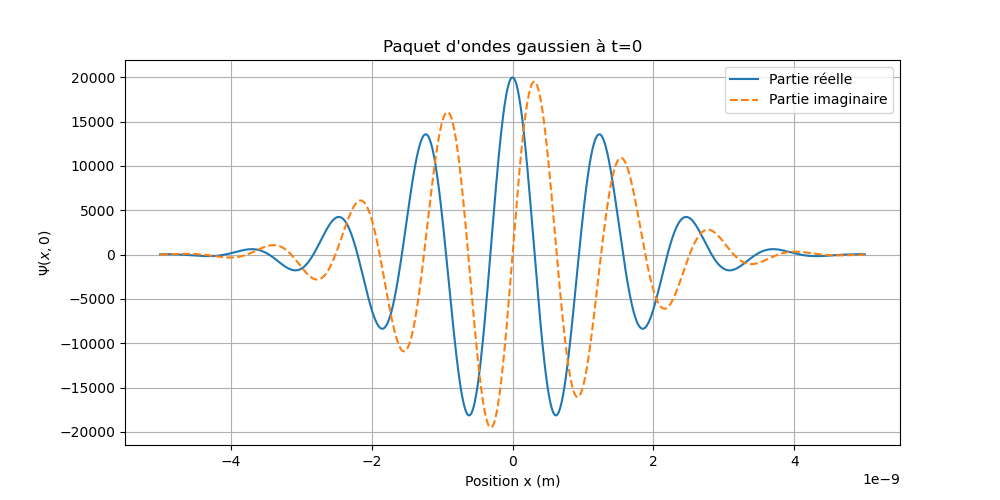
\includegraphics[width=\textwidth]{Figure_0_paquet_re_im.png}
      \centering {\footnotesize Parties réelle et imaginaire à $t=0$ (partie 2).}
    \end{column}
  \end{columns}
\end{frame}

% ------------------------------------------------------------
\begin{frame}{États stationnaires de la barrière rectangulaire}
  Solutions $\psi(x)\,\eg^{-iEt/\hb}$ pour $V(x) = V_0$ sur $[0,a]$, avec $E < V_0$ :
  \[
    \psi_{\rm I} = \eg^{ikx} + R\,\eg^{-ikx}
    \quad\Big|\quad
    \psi_{\rm II} = A\,\eg^{\kappa x} + B\,\eg^{-\kappa x}
    \quad\Big|\quad
    \psi_{\rm III} = T\,\eg^{ikx}
  \]
  \[
    k = \frac{\sqrt{2mE}}{\hb}, \qquad
    \kappa = \frac{\sqrt{2m(V_0 - E)}}{\hb}
    \quad \text{(onde évanescente sous la barrière)}
  \]
  \vspace{0.3em}
  Raccordement de $\psi$ et $\psi'$ en $x=0$ et $x=a$ $\Rightarrow$
  \begin{block}{Amplitude de transmission}
    \[
      T(k) = \frac{\eg^{-ika}}{\cosh(\kappa a)
             + i\,\dfrac{\kappa^2 - k^2}{2k\kappa}\,\sinh(\kappa a)}
      \qquad\Rightarrow\qquad
      |T|^2 = \frac{1}{1 + \dfrac{(\kappa^2+k^2)^2}{4k^2\kappa^2}\sinh^2(\kappa a)}
    \]
  \end{block}
  Régime opaque ($\kappa a \gg 1$) :
  $|T|^2 \approx \dfrac{16k^2\kappa^2}{(k^2+\kappa^2)^2}\,\eg^{-2\kappa a}$
  — décroissance \textbf{exponentielle} avec $a$.
\end{frame}

% ------------------------------------------------------------
\begin{frame}{Méthode numérique : schéma de Crank--Nicolson}
  Équation de Schrödinger discrétisée en moyennant les instants $t_j$ et $t_{j+1}$ :
  \[
    -r\,\psi_{i-1}^{j+1} + (1 + 2r + s_i)\,\psi_i^{j+1} - r\,\psi_{i+1}^{j+1}
    = r\,\psi_{i-1}^{j} + (1 - 2r - s_i)\,\psi_i^{j} + r\,\psi_{i+1}^{j}
  \]
  \[
    r = \frac{i\hb\,\Delta t}{4m\,\Delta x^2}, \qquad
    s_i = \frac{i\,V(x_i)\,\Delta t}{2\hb}
    \quad \text{(diagonale variable : } V(x) \text{ non uniforme)}
  \]
  \begin{columns}[T]
    \begin{column}{0.55\textwidth}
      \textbf{Pourquoi ce schéma ?}
      \begin{itemize}
        \item \textbf{unitaire} : la norme $\int |\psi|^2 dx$ est conservée
              à $10^{-6}$ près sur toute la simulation ;
        \item inconditionnellement stable, précis à l'ordre 2 en temps et en espace ;
        \item système tridiagonal résolu par la méthode de Thomas en $O(n_x)$
              à chaque pas de temps.
      \end{itemize}
    \end{column}
    \begin{column}{0.41\textwidth}
      \textbf{Paramètres de référence :}
      \begin{itemize}
        \item grille : $n_x = 1500$, $n_t = 3000$, $x \in [-30, 30]$, $t \in [0, 6]$ ;
        \item paquet : $k_0 = 5$ ($E = 12.5$), $a_{\rm wp} = 1$, $x_0 = -10$ ;
        \item barrière : $a = 1$, $V_0 = 15 > E$.
      \end{itemize}
    \end{column}
  \end{columns}
\end{frame}

% ------------------------------------------------------------
\begin{frame}{Validation : particule libre ($V_0 = 0$)}
  Mesure des temps par suivi du \textbf{pic} de $|\psi(x,t)|^2$ aux bords de la
  zone $[0, a]$ :
  \[
    \tau_0^{\rm num} = t_{\rm sortie} - t_{\rm entrée}
    \qquad\text{à comparer à}\qquad
    \tau_0^{\rm th} = \frac{a}{v_g} = \frac{m\,a}{\hb\,k_0}
  \]
  \begin{center}
    \begin{tabular}{lcc}
      \toprule
      & numérique & théorique \\
      \midrule
      $t_{\rm entrée}$ (pic en $x=0$)   & 1.9987 & 2.0000 \\
      $t_{\rm sortie}$ (pic en $x=a$)   & 2.1907 & 2.2000 \\
      $\tau_0$                          & 0.192  & 0.200  \\
      \bottomrule
    \end{tabular}
  \end{center}
  \vspace{0.5em}
  \begin{itemize}
    \item Écart de 4\,\% sur $\tau_0$ : résolution temporelle de la grille
          ($\Delta t = 2\times10^{-3}$) et étalement du paquet.
    \item Norme conservée : $0.999999 \to 1.000000$ sur 3000 pas.
  \end{itemize}
  $\Rightarrow$ le solveur est validé, on peut allumer la barrière.
\end{frame}

% ------------------------------------------------------------
\begin{frame}{Évolution face à la barrière}
  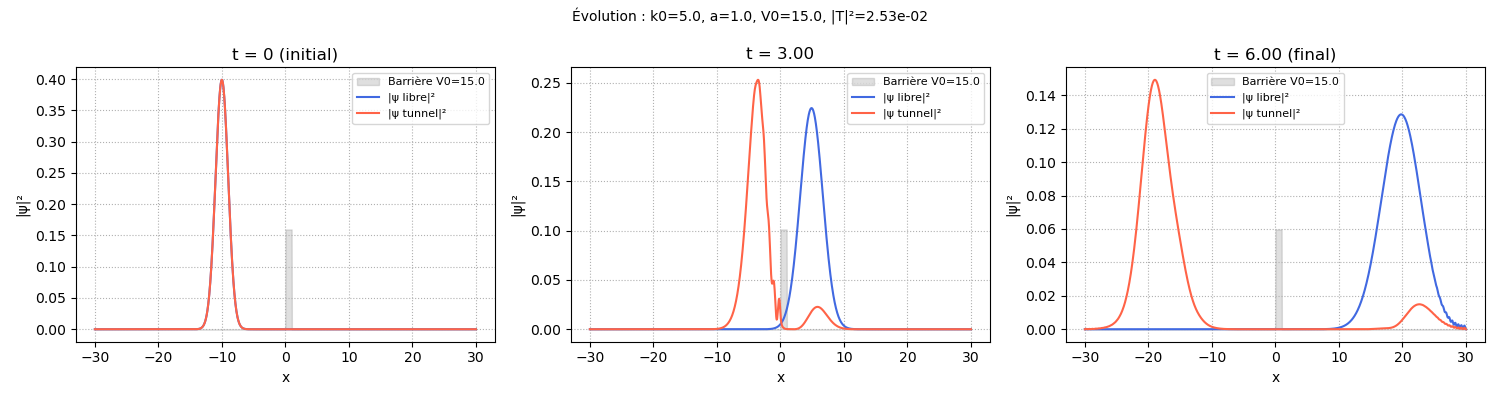
\includegraphics[width=\textwidth]{Figure_1_evolution.png}
  \begin{itemize}
    \item Le paquet incident se sépare en un paquet \textbf{réfléchi} (dominant)
          et un paquet \textbf{transmis} de faible amplitude : l'effet tunnel.
    \item Classiquement, la particule serait réfléchie avec certitude ($E < V_0$).
    \item Comparaison directe avec le paquet libre (bleu) : même $v_g$,
          mais amplitudes très différentes.
  \end{itemize}
\end{frame}

% ------------------------------------------------------------
\begin{frame}{Probabilités de réflexion et de transmission}
  \begin{center}
    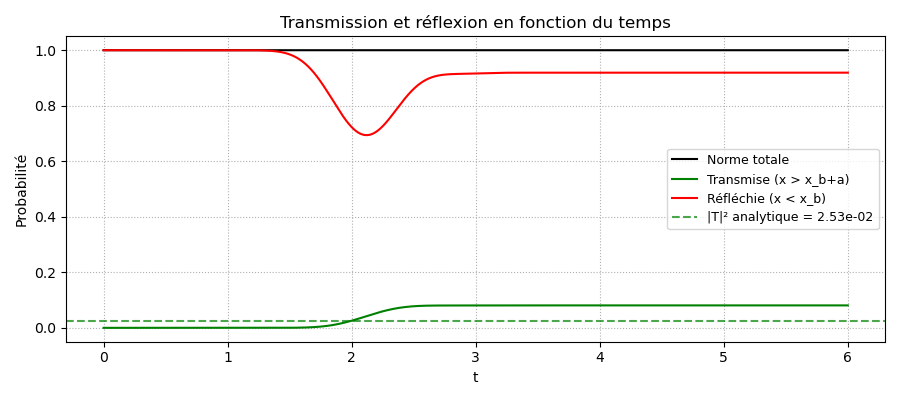
\includegraphics[width=0.78\textwidth]{Figure_2_normes.png}
  \end{center}
  \begin{itemize}
    \item Norme totale constante (Crank--Nicolson unitaire).
    \item Probabilité transmise mesurée : $8.1\times10^{-2}$, contre
          $|T(k_0)|^2 = 2.5\times10^{-2}$ pour l'onde plane.
    \item L'écart n'est pas une erreur numérique : le paquet n'est pas
          monochromatique, et la barrière \textbf{filtre} son spectre
          (nous y reviendrons).
  \end{itemize}
\end{frame}

% ------------------------------------------------------------
\begin{frame}{Quel temps de traversée ? Le temps de groupe de Hartman}
  Le paquet transmis s'écrit en pondérant chaque composante par $T(k)$ :
  \[
    \psi_{\rm trans}(x,t) = \frac{1}{\sqrt{2\pi}}\int g(k)\,T(k)\,
    \eg^{i(kx-\omega t)}\,dk
    \qquad \text{avec } T = |T|\,\eg^{i\varphi_T}
  \]
  Phase stationnaire autour de $k_0$ $\Rightarrow$ le pic transmis est décalé de
  $\tau_g = \dfrac{1}{v_g}\dfrac{d\varphi_T}{dk}\Big|_{k_0}$ \;($< 0$ en régime tunnel) :
  \begin{block}{Temps de traversée théorique}
    \[
      \tau_t^{\rm th} = \tau_0 + \tau_g
      \qquad \text{avec } \varphi_T(k) = -ka
      - \arctan\!\left[\frac{\kappa^2 - k^2}{2k\kappa}\tanh(\kappa a)\right]
    \]
  \end{block}
  \textbf{Résultat} ($k_0=5$, $a=1$, $V_0=15$) :
  $\;\tau_t^{\rm num} = 0.112 \;<\; \tau_t^{\rm th} = 0.168 \;<\; \tau_0 = 0.200$
  — le paquet tunnel sort \emph{plus tôt} que le paquet libre :
  c'est l'\textbf{effet Hartman}.
\end{frame}

% ------------------------------------------------------------
\begin{frame}{Influence de la barrière : largeur $a$}
  \begin{center}
    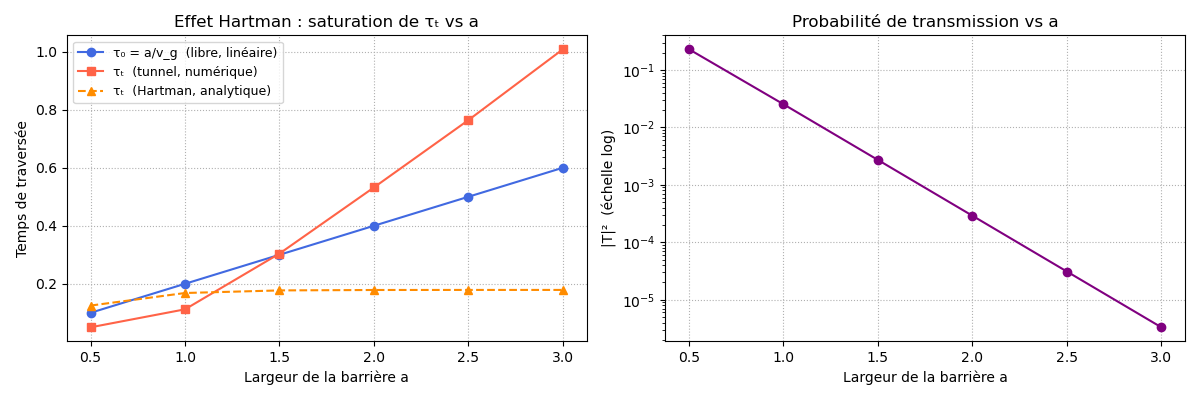
\includegraphics[width=0.82\textwidth]{Figure_3_influence_a.png}
  \end{center}
  \begin{itemize}
    \item $\tau_0 \propto a$ (libre) mais $\tau_t^{\rm th}$ \textbf{sature}
          vers $0.179$ dès $\kappa a \gtrsim 3$ : le temps tunnel devient
          indépendant de l'épaisseur (Hartman, 1962).
    \item $|T|^2$ chute exponentiellement ($\sim \eg^{-2\kappa a}$),
          conformément aux états stationnaires.
    \item Au-delà de $a \approx 1.5$, la mesure par le pic décroche : le
          filtrage spectral domine — limite de cette définition du temps.
  \end{itemize}
\end{frame}

% ------------------------------------------------------------
\begin{frame}{Influence de la barrière : hauteur $V_0$}
  \begin{center}
    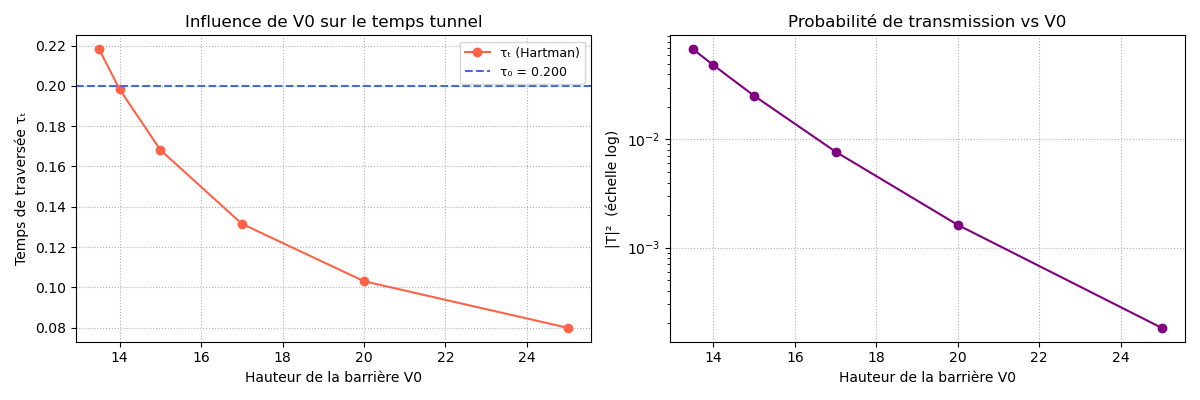
\includegraphics[width=0.82\textwidth]{Figure_4_influence_V0.png}
  \end{center}
  \begin{itemize}
    \item Plus la barrière est haute, plus $\kappa$ est grand : $|T|^2$
          s'effondre\dots{} mais le temps de traversée \textbf{diminue} aussi
          ($0.218 \to 0.080$ pour $V_0 : 13.5 \to 25$).
    \item Résultat contre-intuitif : une barrière plus infranchissable se
          traverse (rarement) mais \emph{plus vite}.
  \end{itemize}
\end{frame}

% ------------------------------------------------------------
\begin{frame}{Influence du paquet : impulsion moyenne $k_0$}
  \begin{center}
    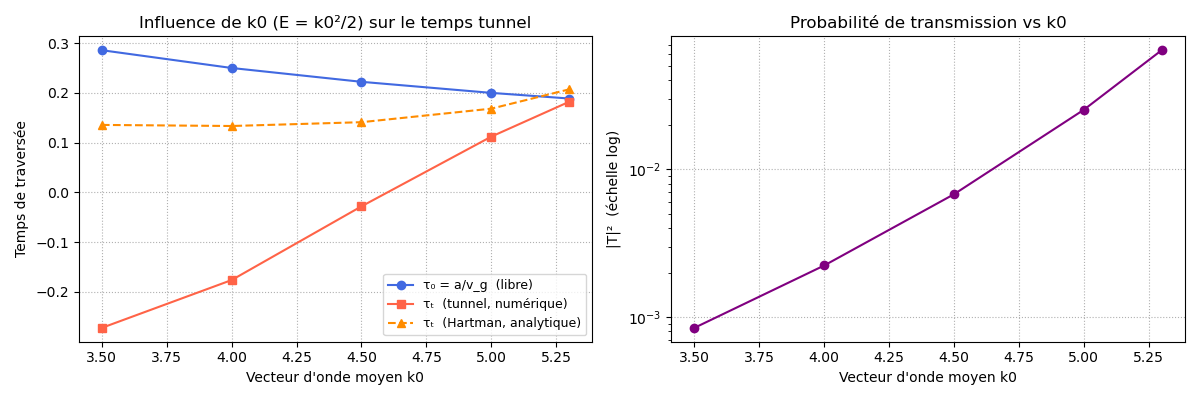
\includegraphics[width=0.76\textwidth]{Figure_5_influence_k0.png}
  \end{center}
  \begin{itemize}
    \item $|T|^2$ gagne deux ordres de grandeur quand $E = k_0^2/2$ se
          rapproche de $V_0$ ; $\tau_t^{\rm th}$ varie peu (0.13--0.21).
    \item Pour $k_0 \lesssim 4.5$, $\tau_t^{\rm num}$ devient \textbf{négatif} :
          le pic transmis sort avant que le pic incident n'entre !
    \item Pas de violation de causalité : seule l'avant-garde rapide du spectre
          est transmise — le « pic » est reconstruit de composantes déjà en avance.
  \end{itemize}
\end{frame}

% ------------------------------------------------------------
\begin{frame}{Influence du paquet : largeur initiale $a_{\rm wp}$}
  \begin{center}
    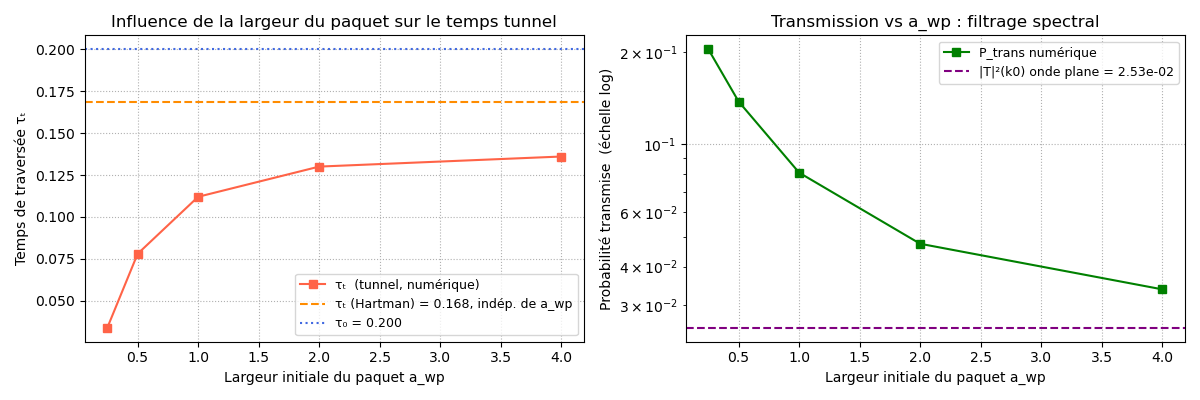
\includegraphics[width=0.76\textwidth]{Figure_6_influence_awp.png}
  \end{center}
  \begin{itemize}
    \item Le temps de Hartman (calculé pour la seule composante $k_0$)
          ne dépend pas de $a_{\rm wp}$ : tout l'écart vient de la largeur
          spectrale $\Delta k = 1/(2\sqrt{a_{\rm wp}})$.
    \item Paquet large ($\Delta k \to 0$) : $\tau_t^{\rm num} \to \tau_t^{\rm th}$
          et $P_{\rm trans} \to |T(k_0)|^2$ — limite quasi monochromatique.
    \item Paquet étroit : les composantes rapides sont favorisées
          $\Rightarrow$ sortie précoce, transmission jusqu'à $8$ fois
          au-dessus de la prédiction onde plane.
  \end{itemize}
\end{frame}

% ------------------------------------------------------------
\begin{frame}{Conclusion}
  \textbf{Ce que nous avons montré :}
  \begin{itemize}
    \item Un solveur Crank--Nicolson validé (norme conservée, $\tau_0$ à 4\,\%
          de la théorie) pour la dynamique d'un paquet gaussien face à une
          barrière.
    \item Les états stationnaires donnent $|T|^2$ et la phase $\varphi_T$ :
          la décroissance exponentielle de la transmission est vérifiée
          numériquement.
    \item Le temps de traversée mesuré confirme l'\textbf{effet Hartman} :
          $\tau_t < \tau_0$, et $\tau_t^{\rm th}$ sature avec la largeur de la
          barrière.
    \item Les caractéristiques du paquet comptent : la notion de temps de
          traversée par suivi du pic n'a de sens que dans la limite
          \textbf{quasi monochromatique} ($\Delta k$ petit) — sinon le filtrage
          spectral domine, jusqu'à des temps apparents négatifs.
  \end{itemize}
  \vspace{0.5em}
  \textbf{Perspectives :} autres définitions du temps tunnel (temps de séjour,
  horloge de Larmor), double barrière, comparaison aux expériences
  d'attophysique.
  \vspace{0.8em}
  \begin{center}
    \emph{Merci de votre attention !}
  \end{center}
\end{frame}

\end{document}
